\section{Architecture}
\label{architecture}

%generall description about the technologies used in the project and how they interact, also why I used the technologies (advantages and disadvantages); also insert figures of the app and throughout this chapter more of each specific activity
As mentioned above, we decided to implement an Android application for mobile phones. Since the Chrome browser offers an interface for using Bluetooth LE on the web, we decided to develop a Chrome extension to utilize their Web Bluetooth API. [link] \\

With the extension, we inject a button on the website. The button is used to establish a Bluetooth LE connection between application and extension. Upon successful pairing, the extension is allowed to read characteristics that are advertised from the app. The characteristics contain username and password, which the extension inserts directly into the login fields of the website. \\

\noindent Before starting with the implementation we defined minimal requirements of the Android application and the Chrome extension: \\

\noindent Minimal requirements of application:
\begin{itemize}
\item Safe storage of credentials (account name, username, and password)
\item Adding, changing and deleting credentials
\item En- and decryption of data 
\item Authentication through biometric identification
\item Establishing a Bluetooth connection with the web extension
\end{itemize}
\vspace{0.3cm}
\noindent Minimal requirements of extension:
\begin{itemize}
\item Injection of a button onto the website
\item Establishment of Bluetooth LE Connection
\item Reading the advertised characteristics
\item Filling credentials into the proper login fields
\end{itemize}


%technical details:
\noindent For convenience purposes, we implemented the application for API level 23 minimum and up using Android Studio as the IDE. To go more into detail about the app, it consists of a main activity [ref figure 1], which contains four different menu items: \textit{Accounts}, which provides the user with an interface to manage their login accounts; \textit{Connection}, where users can establish the Bluetooth connection and send their login data to the web browser; \textit{Settings} and \textit{About}. We will go more into detail about the functionality of the activities \textit{Accounts} and \textit{Connection}. Subsequently, we will examine how the application handles data storage, encryption, and authentication in greater detail. \\

\begin{figure}[H]
\centering
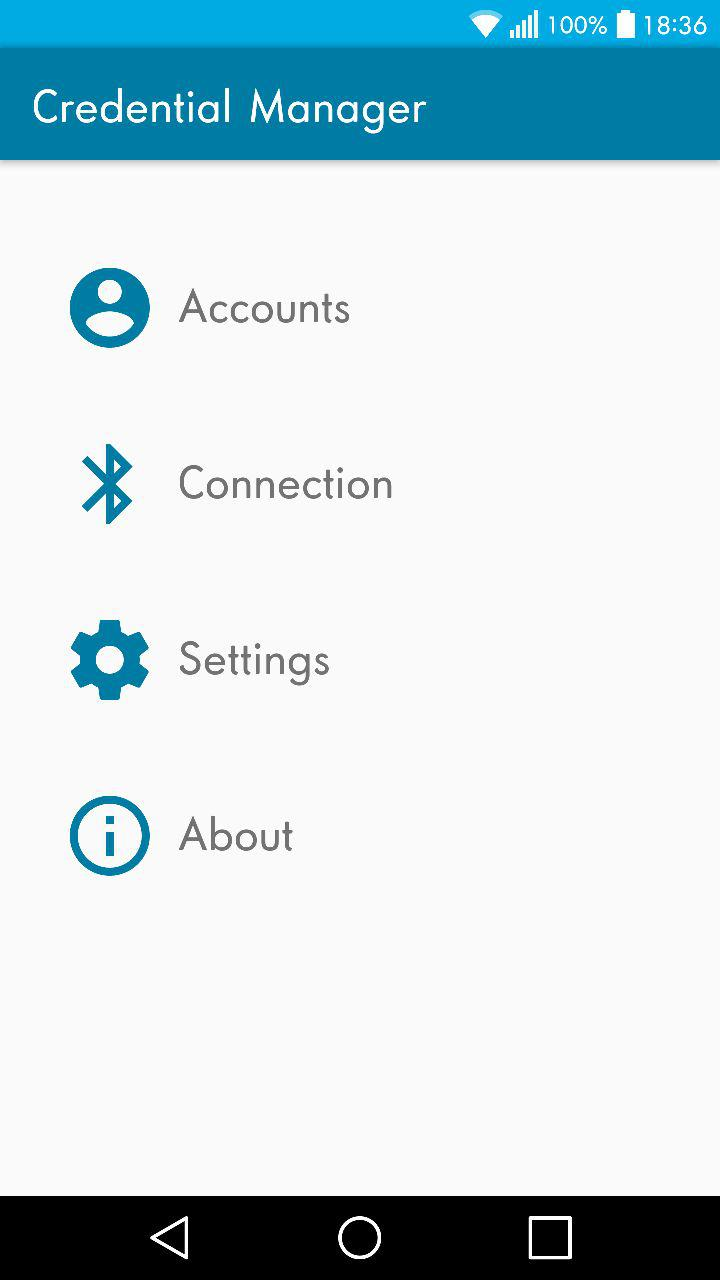
\includegraphics[width=6cm]{images/MainActivity}
\caption[Main activity]{Main activity, which is shown at start up of the app}
\label{fig:mainactivity}
\end{figure}

%-------------------------------------------------------------------------------------

\subsection{Activity for managing Accounts}
By clicking on the menu item \textit{Accounts}, the user is asked to authenticate themselves using biometric information in the form of fingerprint or a master password as seen in figure \ref{fig:authentication}\protect\subref{auth_screen}. Upon successful verification, the interface is shown where the user has an overview of his saved credentials as seen in Figure \ref{fig:accountactivity}\protect\subref{show_acc}. By clicking the button on the bottom right corner, the activity is switched and the user can add a new login as seen in Figure \ref{fig:accountactivity}\protect\subref{add_acc}. The user types in the website to which username and password belong to as well as the username and password. Clicking the save-button encrypts and adds the credential to the database. \\

When clicked on one of the existing credentials in the list, it takes the user to the interface shown in Figure \ref{fig:accountactivity}\protect\subref{change_acc}.  Here the values can be changed and saved again, or the login account can be deleted from the database. When deleting a credential, the user will be asked via a prompt as seen in Figure \ref{fig:accountactivity}\protect\subref{prompt_delete}.

\begin{figure}[H]
\centering
\subfloat[]{{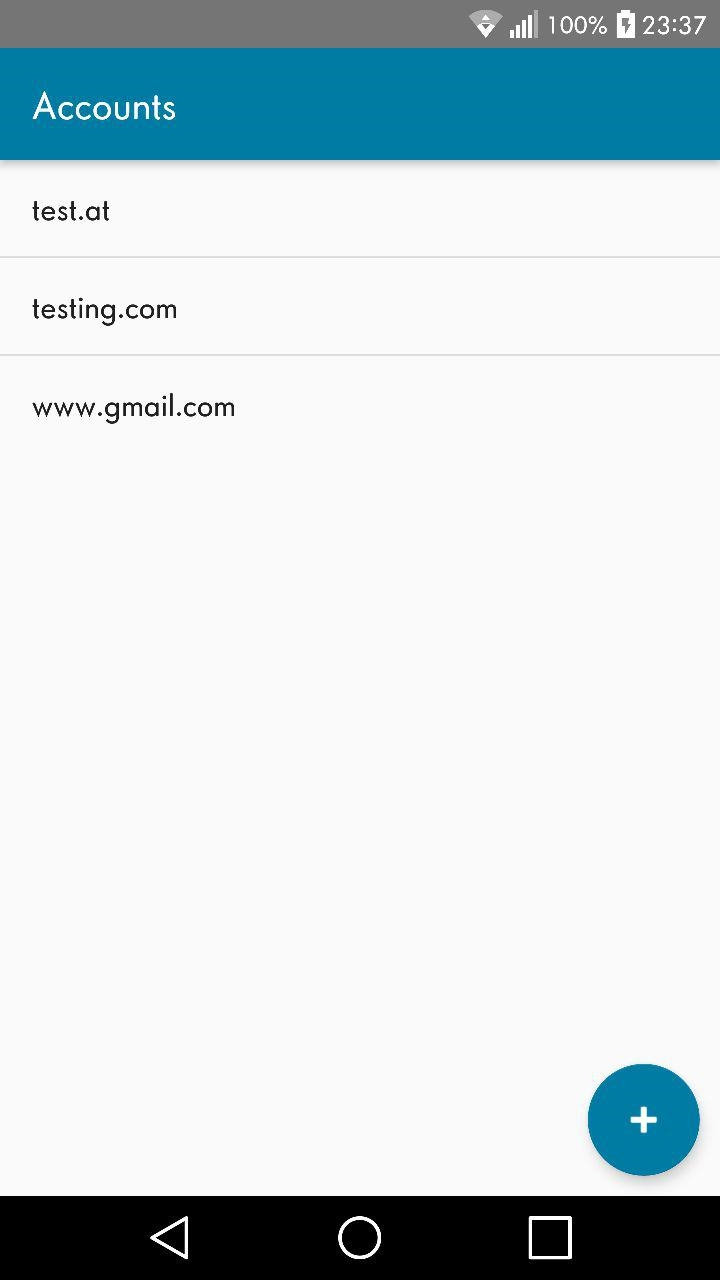
\includegraphics[width=4cm]{images/ShowAccountsActivity}\label{show_acc} }}
\qquad
\subfloat[]{{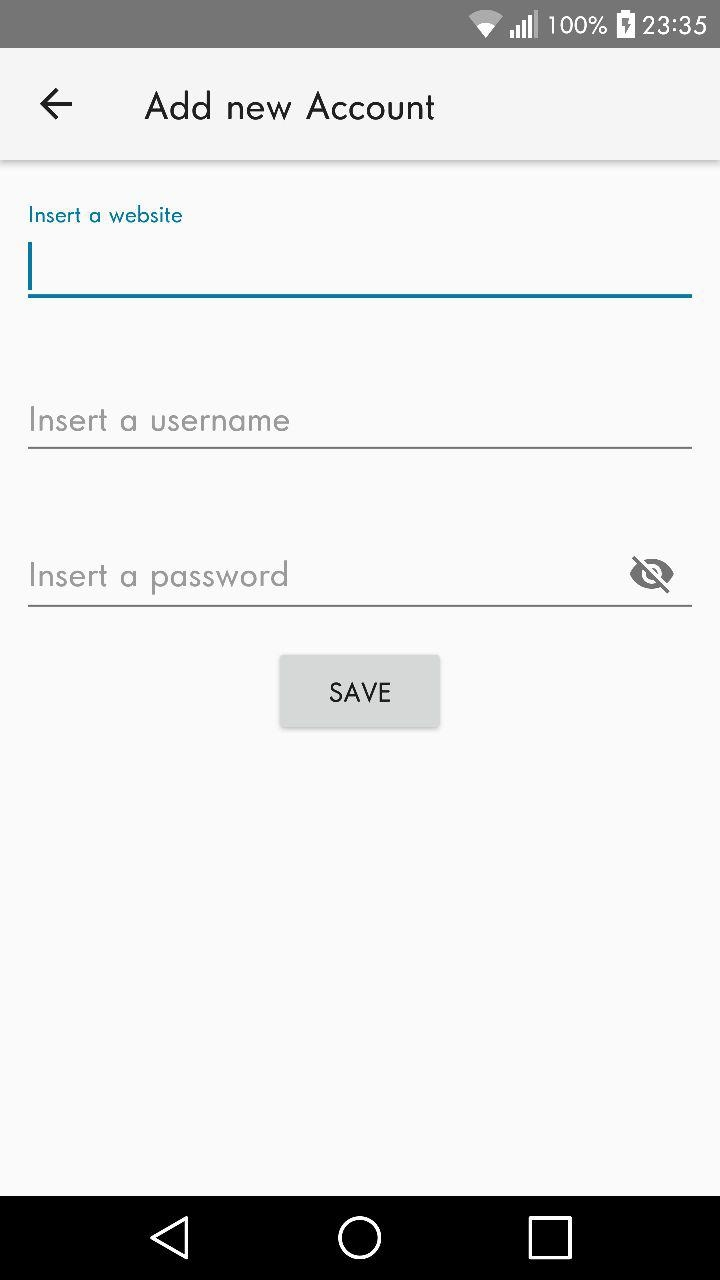
\includegraphics[width=4cm]{images/AddAccountActivity}\label{add_acc} }}
\qquad
\subfloat[]{{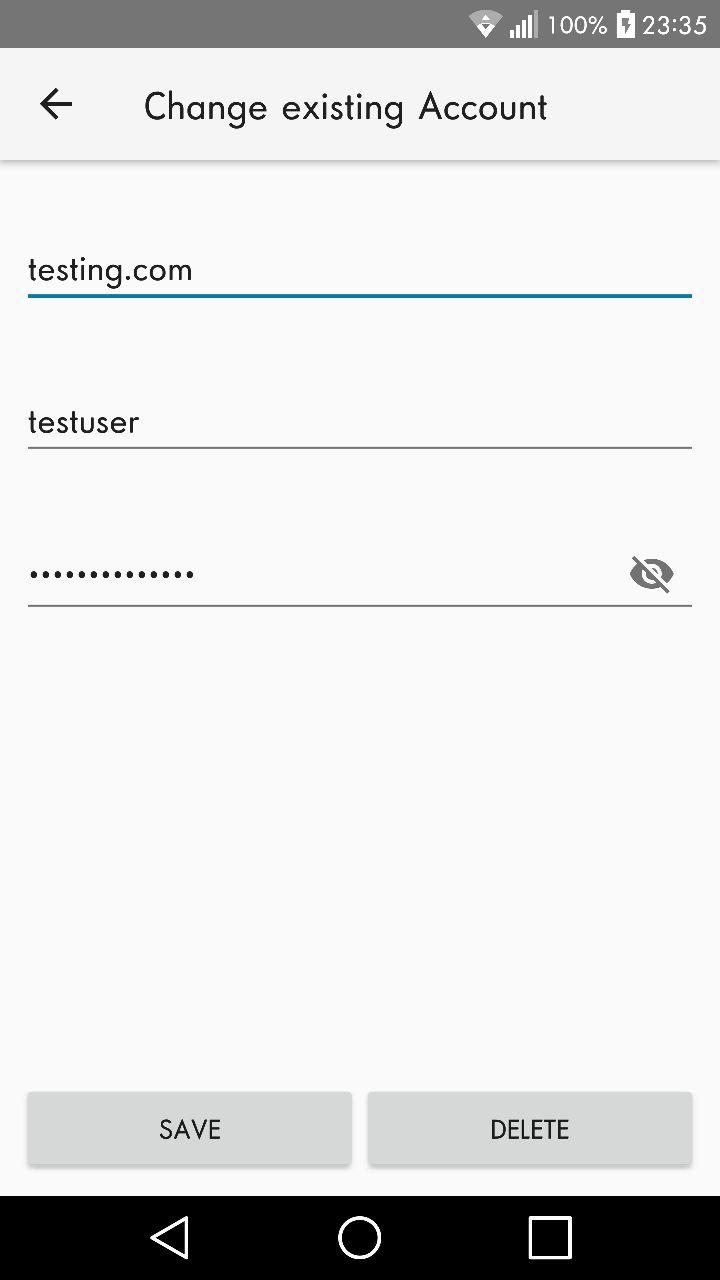
\includegraphics[width=4cm]{images/ChangeAccountActivity}\label{change_acc} }}
\qquad
\subfloat[]{{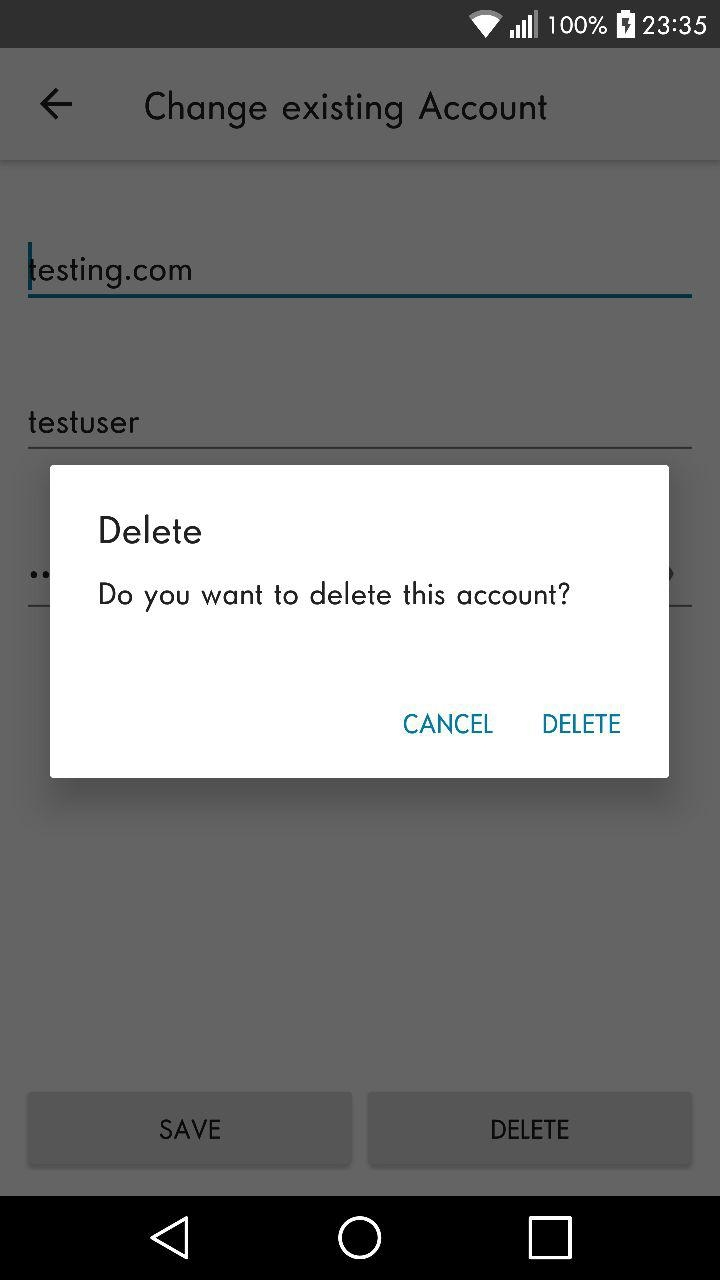
\includegraphics[width=4cm]{images/DeleteAccount}\label{prompt_delete} }}
\caption[Activity for managing Accounts]{Activity for managing Accounts: In \protect\subref{show_acc} it shows the listed accounts after success user authentication. \protect\subref{add_acc} is the interface where the user can add accounts and in \protect\subref{change_acc} the user can change a selected account. \protect\subref{prompt_delete} asks the user before deleting credentials out of the database.}
\label{fig:accountactivity}
\end{figure}

%-------------------------------------------------------------------------------------

\subsection{Activity for Bluetooth Connection}
After selecting the menu item \textit{Connection}, the app checks immediately if Bluetooth is enabled. If it is not turned on, the user is asked via prompt to enable Bluetooth as shown in Figure \ref{fig:connectionactivity}\protect\subref{prompt_bt}.
If the activation is denied, then the application will return to the main activity with an error message displayed in Figure \ref{fig:connectionactivity}\protect\subref{bt_notEnabled}. \\

Once Bluetooth is enabled, the accounts available for sharing are listed.
At first, the application does not advertise any data. The user is asked to select an account to send to the Web Bluetooth API as seen in Figure \ref{fig:connectionactivity}\protect\subref{not_advertising}. Before any credentials are shared, the user is asked to authenticate himself using his fingerprint or his master password. Figure \ref{fig:connectionactivity}\protect\subref{advertising} shows that only after successful authentication the advertising starts and the Web Bluetooth API searches for BLE devices that are near.

\begin{figure}[H]
\centering
\subfloat[]{{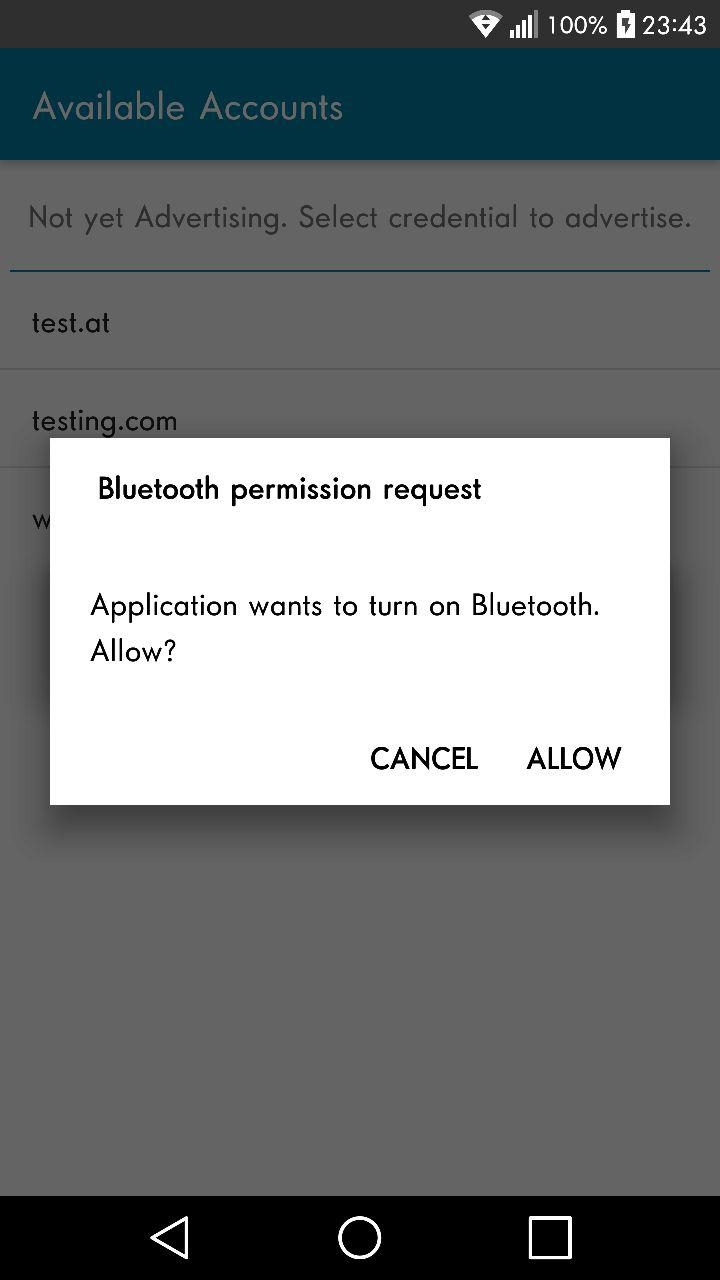
\includegraphics[width=4cm]{images/BT_english}\label{prompt_bt} }}
\qquad
\subfloat[]{{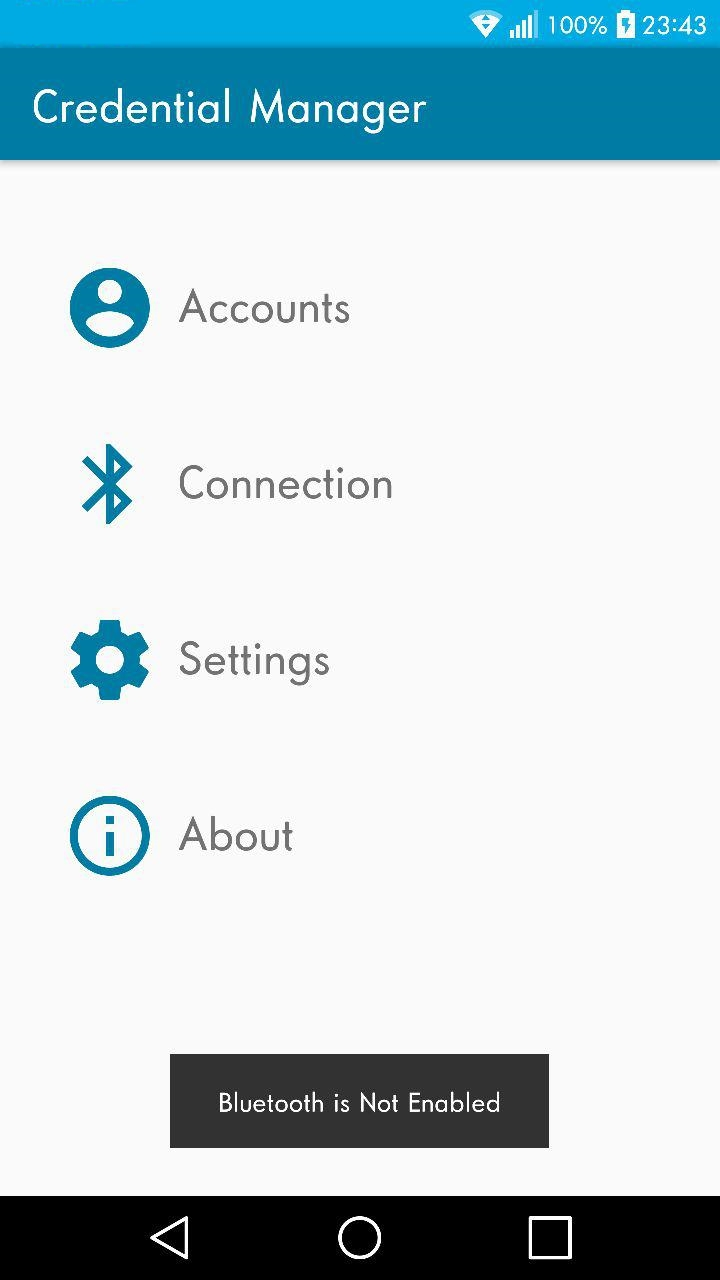
\includegraphics[width=4cm]{images/BTNotEnabled}\label{bt_notEnabled} }}
\qquad
\subfloat[]{{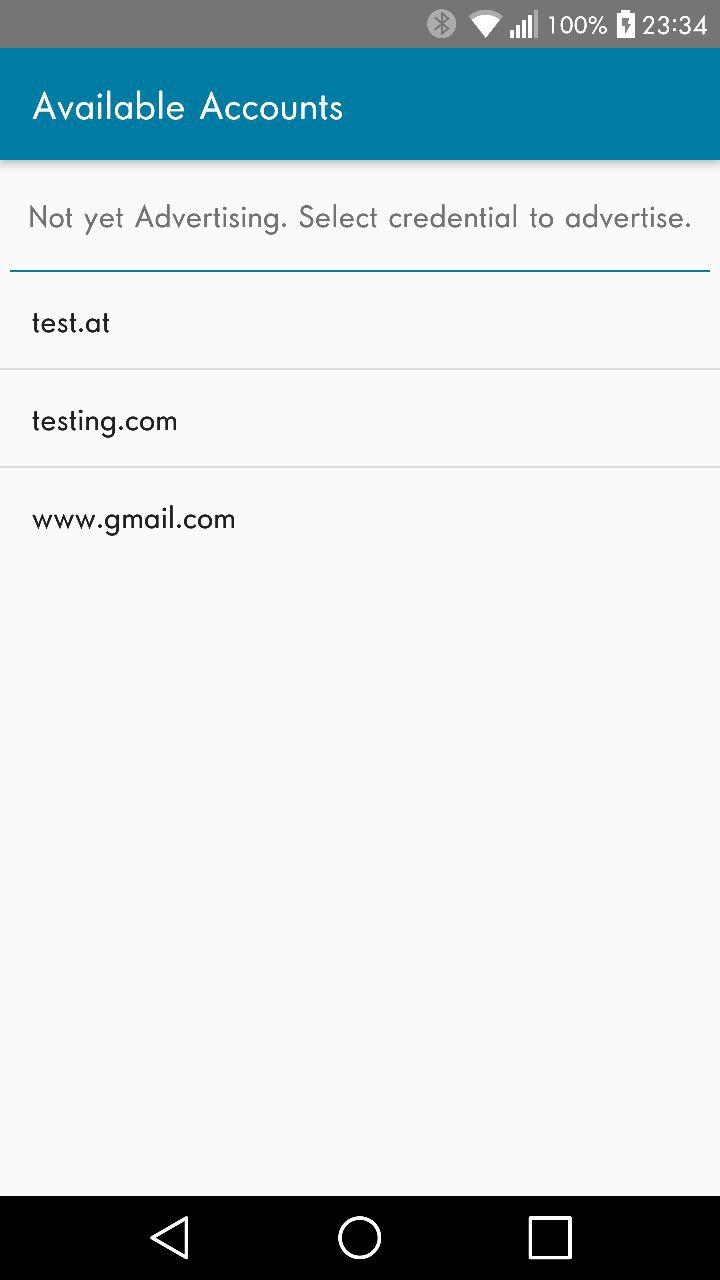
\includegraphics[width=4cm]{images/AvailableAccounts}\label{not_advertising} }}
\qquad
% !!!!!!!!!!!!! change jpg once programming done and working!
\subfloat[]{{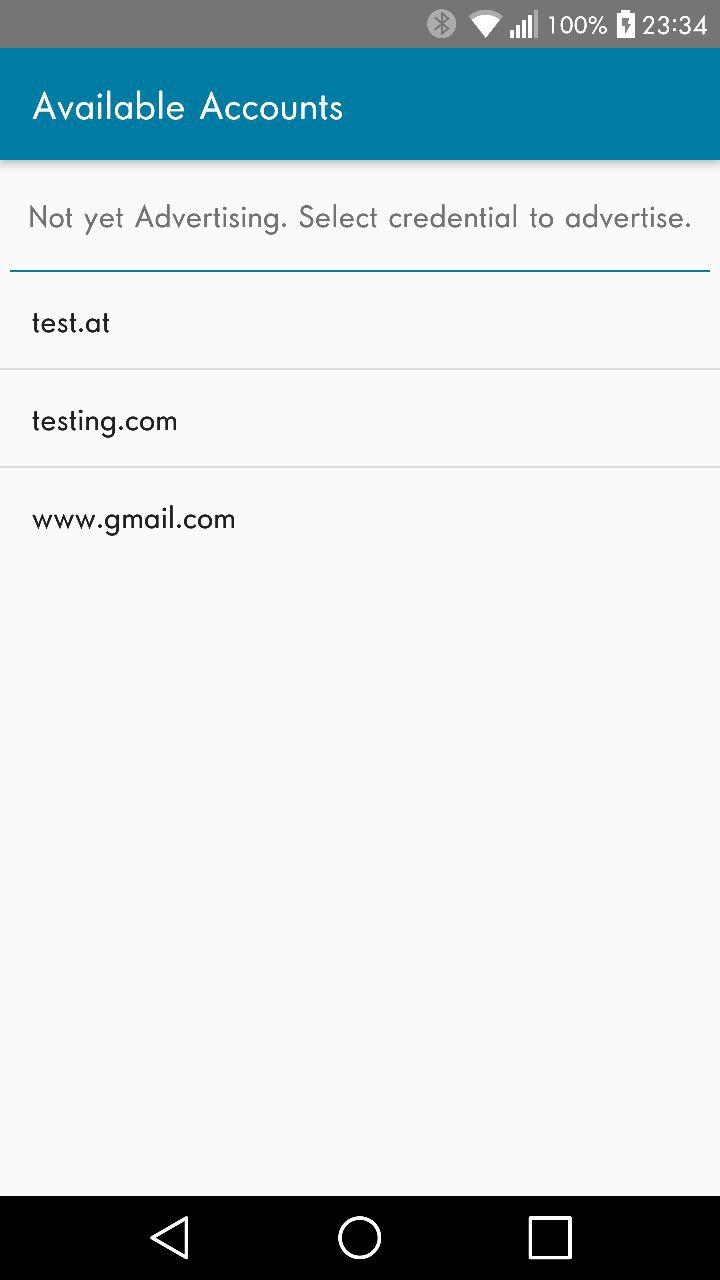
\includegraphics[width=4cm]{images/AvailableAccounts}\label{advertising} }}
%\qquad
%\subfloat[Asking the user before deleting the credential out of the database]{{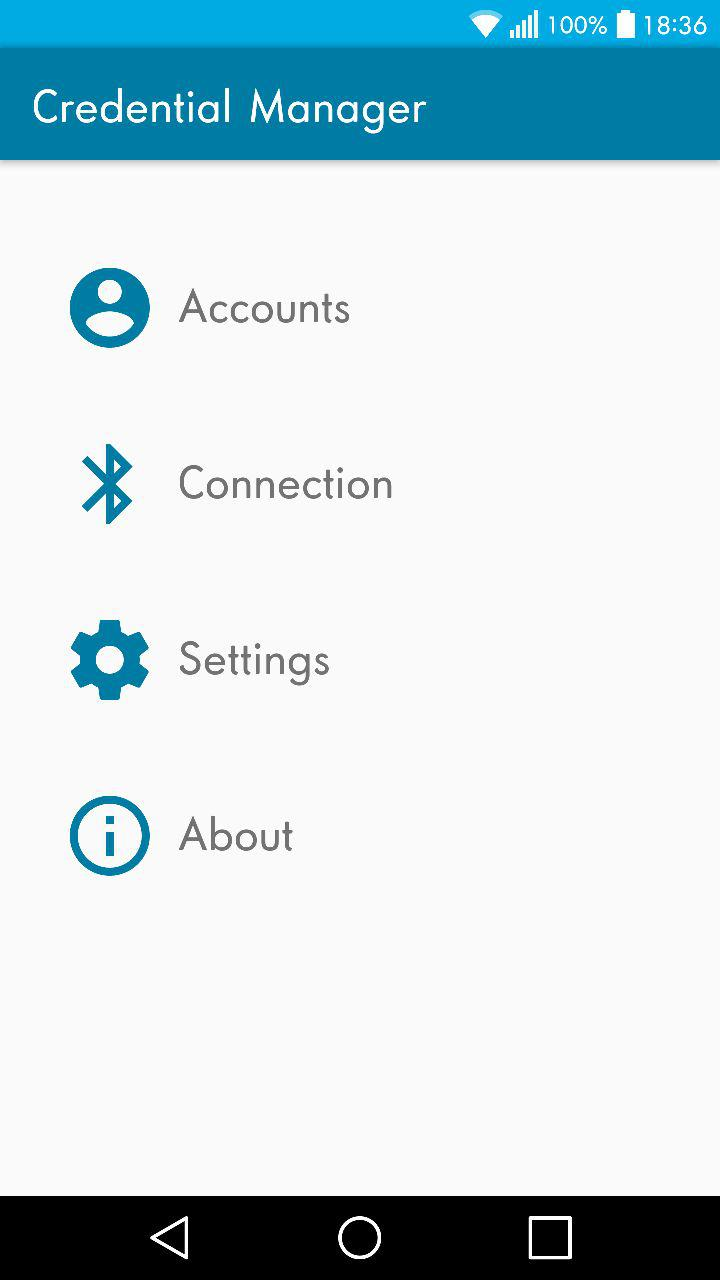
\includegraphics[width=5cm]{images/MainActivity} }}
\caption[Activity for Bluetooth Connection]{Activity for Bluetooth Connection: In \protect\subref{prompt_bt} a prompt is shown to the user to enable Bluetooth. When the application is not advertising, \protect\subref{not_advertising} is shown and \protect\subref{advertising} is shown after user selected a credential to send.}
\label{fig:connectionactivity}
\end{figure}

%-------------------------------------------------------------------------------------


\subsection{Storage using greenDao ORM}
Since the goal is to store user credentials on the phone,  we need a suitable database structure. One option was using a common SQLite database, which is widely used for Android applications. SQLite databases use, as conventional SQL databases, SQL queries to store, retrieve and delete data. However, SQL queries can be vulnerable to security attacks, for example, second-order SQL injections. As stated in [Detection of SQL Injection Attacks] a SQL injection is defined as a method where code is injected. This exploits a security vulnerability in the database layer of an application. It is done by modifying input data which then alters the SQL query. This procedure increases the risk of storing data safely and may lead to a vulnerable application. In [Detection of SQL Injection Attacks] it is also stated that the risk of a SQL injection attack can increase due to not investing sufficient development time or lack of experience and knowledge. Therefore, we decided not to implement traditionally SQL queries.

For this project, we decided to use an object/relational mapping. It manages the tasks of storing, deleting, updating and querying, while saving time and resources. We decided on the greenDAO ORM [ref http://greenrobot.org/greendao/] as it has an overall good performance. Additionally, it does not require as much programming effort compared to other frameworks as discussed in [ref greenDAO paper]. \\

Before we started with setting up the database we needed to included the greenDAO plugin into the project. [greendao link] Next step was the set up the database. This was done by initializing a DaoSession which is given by a DaoMaster. The DaoMaster was provided from the helper class \texttt{DevOpenHelper}, which we instantiated as shown in Listing \ref{lst:db_master}.

\begin{lstlisting}[caption=Creation of database, label=lst:db_master]
DaoMaster.DevOpenHelper helper = 
        new DaoMaster.DevOpenHelper(this,"credentials-db");
Database db = helper.getWritableDb();
daoSession = new DaoMaster(db).newSession();
\end{lstlisting}
\vspace{0.5cm}

The DaoMaster handles the database set up and creates DaoSessions. A DaoSession, on the other hand, manages the DAO object. It is an entity that we store into the database. DAO objects are created from a Java class with annotations. The class we used holds four members: a unique id, the website, username, and password. To define a Java class as a database-backed entity, annotations to the class-header as well as to the class members must be added. The class members define the columns of the database. Afterward, the greenDAO generator automatically generates required methods. After this process, instances of the class can be stored into the greenDAO database. [link greendao]. \\

\subsubsection*{Load, insert and delete a database entry}
As mentioned before, the DaoSession manages DAO objects and they, in turn, handle all operations of the database. With the start of the application, the database is opened, and a new DaoSession is instantiated.
Additionally, we defined a database helper class where the interactions of DAO objects and the database take place. \\
Listing \ref{lst:db_insert} shows an example of how one credential is inserted into the database. The DaoSession calls the DAO object, and the object handles the insert method to store data into the database. The load and delete methods use the DaoSession as well. \\


\begin{lstlisting}[caption= Insert entry into database, label=lst:db_insert]
public void insertNewAccount(Account account) {
    AccountDao accountDao = this.daoSession.getAccountDao();
    accountDao.insert(account);
}
\end{lstlisting}
\vspace{0.5cm}


The database created by the application lies on presistent memory of the mobile device, and can only be accessed from our app. Even if the database content is dumped in case of an attack, the attacker only receives encrypted data. In section \ref{arch_encryption} we discuss how data is encrypted before inserting into the database and decrypted again when fetching from it.

%-------------------------------------------------------------------------------------

\subsection{Encryption of Data}\label{arch_encryption}
%explaining the en and decryption of data, all about choosing a key: all about cipher and algorithm, code lines and android developer cites, modes paddings usw.
For en- and decryption of sensitive data there exist different possibilities. One option of storing passwords is hashing it and storing the hash in the database. SHA256 or SHA512 are some hash algorithms as mentioned in [Implementation and Performance Analysis of PBKDF2]. By hashing data for encryption, data can be recovered by multiple different attacks such as Brute Force or Dictionary attack.
Another way to store sensitive data is to hash it with a random string of bits, called \textit{salt}. It is stored with the hash of the plaintext. This can also become vulnerable to the Dictionary Attack as stated in [https 3 wrong ways to store a password].
Nowadays it is common to use a key derivation function to safely store passwords. They must generate a strong key that is secure against attacks. Latest key derivation functions are \textit{password-based key derivation function 2 (PBKDF2)}, \textit{Bcrypt}, and \textit{Scrypt}. As mentioned in [ref pbkdf2 secure for passwords], their security is strong.
PBKDF2 requires the user's input to generate the key for encryption. Therefore, the generated key will depend on the password chosen by the user. [https://blog.agilebits.com/2014/03/10/crackers-report-great-news-for-1password-4/] As mentioned before, more than 90\% of users chose a password that is not very safe. In case of a very simple password, PBKDF2 cannot perform as securely as with a secure master password. [ref 3 wrong ways]. Therefore, we need a way to provide safe en- and decryption without depending on the user's ability to create a secure password. \\

Also, all encryption takes place within the mobile phone, and there is no need for any public encryption component. Therefore, encryption and decryption could be done with the same key. [evaluating the perf of symmetric encry algo.] We decided to encrypt data using the AES algorithm. The AES algorithm is a symmetric key algorithm which encrypts data in 128-bit blocks with the generated key. [128vs256] Also, the symmetric encryption scheme is faster than an asymmetric algorithm.\\

We used the Galois/Counter Mode (GCM) as our cipher mode. GCM uses the Counter Mode (CTR) internally. [https://proandroiddev.com/security-best-practices-symmetric-encryption-with-aes-in-java-7616beaaade9] A counter value for each block is encrypted and only uses as many bits as required from the last block. Hence, it turns the block cipher into a stream cipher, and no padding is required. %[https://crypto.stackexchange.com/questions/26783/ciphertext-and-tag-size-and-iv-transmission-with-aes-in-gcm-mode]
We instantiated the cipher, as seen in Listing \ref{lst:cipher}.

\begin{lstlisting} [caption=Instantiation of cipher, label=lst:cipher]
final Cipher cipher = Cipher.getInstance("AES/GCM/NoPadding");
\end{lstlisting}


The GCM provides confidentiality, integrity, and authenticity for securing data. [https://proandroiddev.com/security-best-practices-symmetric-encryption-with-aes-in-java-7616beaaade9] Hence, it is ideal for generating a secret key that is also independent of user data.

For encryption, GCM takes the inputs IV, plaintext, and additional authenticated data (AAD). The AAD is not required and does not affect the security of the GCM mode. []%[https://crypto.stackexchange.com/questions/35727/does-aad-make-gcm-encryption-more-secure].
In this project, we passed the plaintext and the IV. The output of encryption is the ciphertext and an authentication tag. [nist gcm] The authentication tag contains information, that is associated with the data encrypted. It is useful in case of unauthorized change to the encrypted data. [] %[https://proandroiddev.com/security-best-practices-symmetric-encryption-with-aes-in-java-7616beaaade9]
When decrypting data, GCM expects the IV, a ciphertext, the authentication tag, and the AAD, if it has been passed during encryption.
Only if the authentication tag calculated during encryption and then passed one are identical, the plaintext is returned. [nist gcm] \\

Important for the Android implementation of GCM is the length of the initialization vector (IV). National Institute of Standards and Technology recommends 96 bits for the IV to be fast and secure. [Recommandations GCM] [link] To ensure that a unique IV is used with every encryption, a new one is generated upon each call of the encrypt method. Afterward, we concatenate the IV to the ciphertext. Before decryption, the IV is separated from the ciphertext again. We created the IV using the strong random number generator (RNG) \textit{SecureRandom} from the Android Library [https://developer.android.com/reference/java/security/SecureRandom]. \\

A problem occurred when calling the method \texttt{cipher.doFinal(cipherText)} while using the SecureRandom class to generate our IV. 
Android insists on using their method \texttt{cipher.getIV();} for generating the IV. Ref[]%[https://doridori.github.io/Android-Security-Beware-of-the-default-IV/#sthash.Mc8Vyc0J.ED6pvZ9x.dpbs]
argues that using the default IV may not be secure because of risk of reusage. Reusing an IV results in a vulnerable implementation and compromises the security of data. The IV being unique is almost as important as the key being secret. [nist gcm] Therefore, we decided to provide the IV by a SecureRandom instead of using the default method. Android believes we may be working unsafely, because we are not using the provided method \texttt{cipher.getIV()}. To solve the problem, we set the \textit{setRandomizedEncryptionRequired()} property to \textit{false} when we generated the key, which is shown in Listing \ref{lst:key}. This way Android allows using the generated SecureRandom as the IV. []
%[https://medium.com/@ericfu/securely-storing-secrets-in-an-android-application-501f030ae5a3]

\begin{lstlisting} [caption=Setting properties of secret key, label=lst:key]
SpecBuilder.setKeySize(128)
    .setBlockModes(KeyProperties.BLOCK_MODE_GCM)
    .setEncryptionPaddings(KeyProperties.ENCRYPTION_PADDING_NONE)
    .setRandomizedEncryptionRequired(false);
\end{lstlisting}


After generation of the key and successful encryption, it is crucial to store the key securely. We rely on the Android Keystore for this task. Chapter \ref{arch_keystore} discusses the safe storage of the key.


%maybe put pieces of console to show what is effectivly store into the data base and how it is retrieved and decrypted again?

%-------------------------------------------------------------------------------------

\subsection{Secure Storage of Secret Key} \label{arch_keystore}
%explaining what it done with the key afterwards, after creation, how can it be safely stored and not revealed, tee never leaves phone and if then it is destroyed, attacker is only left with encrypted dump of DB, without key cannot retrieve plaintext; what is the tee, where is it, how is it managed and is it on every phone? which phones?
As stated in ref[nist gcm] and [paper analysis of secure key storage solutions on android],  in practice the secrecy of the key and secure storage are crucial. If the key can be retrieved from the device, the data's security is exceedingly compromised. With the key, all ciphertexts can be decrypted easily. Therefore, we need a system to ensure safe storage of the key. \\

The \textit{AndroidKeystore} system allows safe storage of cryptographic keys. Applications use this Android Framework API  to access Keystore functionality. [https://source.android.com/security/keystore/] The AndroidKeystore lets an app store and manage its credentials while making sure no other application can access them. [androidkeystore] \\

To increase the security of the key, we made use of the hardware-based security feature provided by a specific realization of the AndroidKeystore. Modern mobile phones' processors are equipped with ARM TrustZone Technology. [paper analysis of secure key storage solutions on android] This technology separates the hardware into a secure world OS and normal OS. The secure world OS is also known as a Trusted Execution Environment (TEE). The TEE ensures that data does not get leaked out of this trusted environment. Hence, keys stored in the TEE cannot be retrieved. Utilization of the TEE depends on the device manufacture. On devices equipped with a Qualcomm processor with TrustZone Technology, the AndroidKeystore is stored in the TEE. [paper analysis of secure key storage solutions on android] This represents the most secure option to store keys. [https://proandroiddev.com/secure-data-in-android-encryption-in-android-part-1-e5fd150e316f] If TEE is not supported, the keys are stored in a system provided emulated software environment. However, keys will be removed when deleting the application that created them. \\

Before we can generate a key or use it for encryption, we must instantiate and load the Keystore.
A key is stored into the Keystore under a given identifier, also known as \textit{alias}. [paper analysis of secure key storage solutions on android] The alias is a string that defines a reference to the key. All cryptographic operations are done in the background, and key material is never exposed. Hence, the alias is needed everytime data is en- and decrypted. \\

Also, the lock screen must be set in order to reference the key. The KeyguardManager is used for this process. The method \texttt{isDeviceSecure()} returns if the device is secured with a PIN, pattern or password.[https://developer.android.com/reference/android/app/KeyguardManager]
If the device is not locked, the AndroidKeystore is not instantiated, and cryptographic calculations cannot take place. \\




%-------------------------------------------------------------------------------------

\subsection{Authentication through Biometrics}
To securely protect the access and sending of user credential the app uses biometric authentication in the form of fingerprint scanning. The application does not store any biometric user information into the database. Rather, it retrieves the already saved fingerprints on the Android mobile phone. This way it ensures that only the owner of the mobile phone has access to the credentials and the app does not have to handle the storage of any fingerprints. In addition the application also checks if a fingerprint sensor is available on the device and if the permission to use fingerprint scanning is granted from the Android permission system. (maybe ref to chap.6.2 more details about permission system). \\
Before starting authentication via fingerprint the application makes sure that the lock screen is secured by a PIN, password, pattern or if the SIM card is locked. This is done by the \texttt{KeyguardManager} because if provides access to the lock screen. Only in case of a secured mobile device the authentication process will proceed. \\

The application checks if the saved fingerprints contain the one that the user scanned and returns a successful authentication. Otherwise, it throws an error saying that the authentication failed.  If the phone does support fingerprint scanning, but there are no fingerprints stored on the device, the application returns an error message saying that the user must save at least one fingerprint onto the device. If the phone does not have a fingerprint sensor to support scanning mechanism the user has the option of entering a master password, which is set upon the first usage of the application. 

As mentioned above, upon every request to send an account login the user has to re-authenticate using his fingerprint or a master password before sharing credentials with the Web Bluetooth API. This security mechanism would prohibit unwanted distribution of sensitive data if the user left their phone unattended with the phone unlocked and the application still running.

%insert code listing to see how cipher is created??


\begin{figure}[H]
\centering
\subfloat[]{{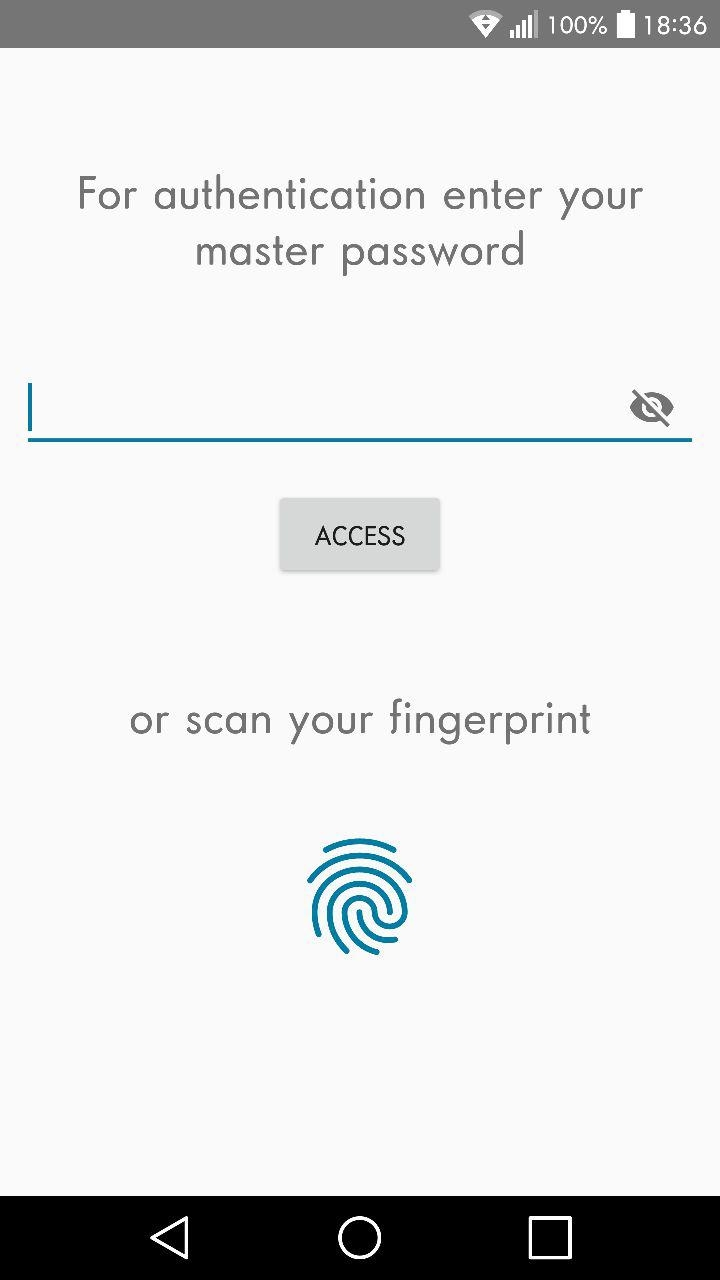
\includegraphics[width=4cm]{images/AuthenticationScreen}\label{auth_screen} }}
\qquad
\subfloat[]{{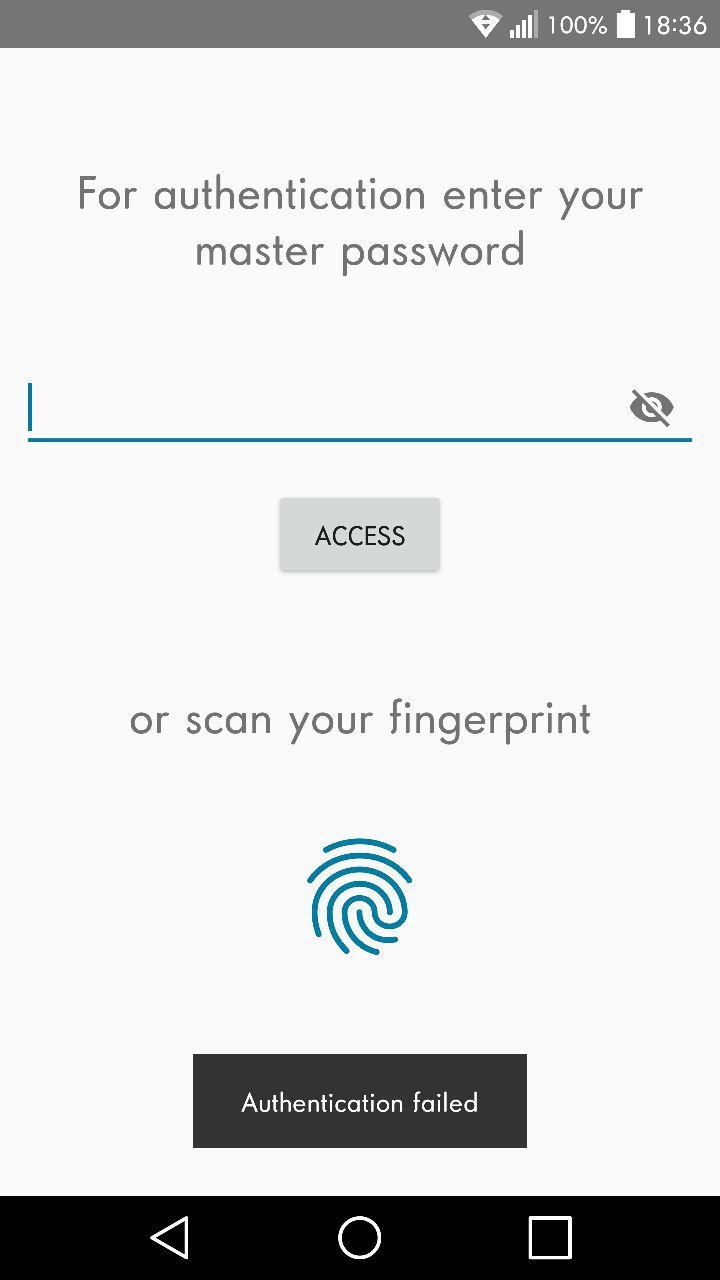
\includegraphics[width=4cm]{images/AuthenticationFailed}\label{auth_fail} }}
\caption[Activity for Authentication]{Activity for Authentication: In \protect\subref{auth_screen} the user is asked to auhenticate themselves using fingerprint or a master password. In \protect\subref{auth_fail} authentication failes if incorrect fingerprint is scanned.}
\label{fig:authentication}
\end{figure}

%-------------------------------------------------------------------------------------

\subsection{Using the Web Bluetooth API with Chrome extension}
 searches for BLE devices that are near and offer a specific service that is defined through a UUID, a universally unique identifier. 
 
%-------------------------------------------------------------------------------------
 

\subsection{Peripheral and Central roles}
After discussing in depth the credential storage, encryption and the authentication of the user, we will briefly describe the roles of the extension and the Android application.

In common use cases, the Android application has the central role in a Bluetooth LE connection, for example when communicating with Bluetooth LE devices, such as a heart rate monitor or beacon. Therefore, the app serves as the client while the Bluetooth LE device acts as the server, sending data that the application wants to receive.

In this scenario, however, the roles are reversed. The Android app serves as the server, where it advertises the data that the Bluetooth LE extension wants to read. Consequently, the application opens a GATT server to advertise the characteristics and the extension, on the other hand, acts as the client and retrieves those advertised characteristics from the app. The extension implements a GATT service and reads the values from the characteristics, which are the login credentials.

